
\begin{definition} [Grafica de $f$] 
\label{def:grafica}
 \mbox{}
 
Sea $f: A\subseteq\Re^n\rightarrow\Re$; se define la gráfica de $f$; y se nota $graf(f)$; a
 \[
graf(f)=\{(x_1,x_2,...,x_n,x_{n+1})\in\Re^{n+1} \backslash (x_1,x_2,...,x_n)=A \land f(x_1,x_2,...,x_n)=x_{n+1} \}
 \]

Para interpretar esta definición, podemos realizar un recuerdo a Análisis matemático 1, donde la $graf (f)$ de una funcion $f: A\subseteq\Re\rightarrow\Re$ se define como
 \[
graf(f)=\{(x,y)\in\Re^2 \backslash x\subseteq A=Dom(f) \land y=f(x) \}
 \]
Planteamos de ejemplo: $f=x^2-1$ donde podemos ver que para cada valor de $x$, existe un único valor de y. Para encontrar la gráfica de la funcion, nos fijamos utilizando la siguiente tabla
\begin{table}[h!]
\centering
\begin{tabular}{|c|c|}
\hline
\textbf{$x$} & \textbf{$f(x)$}  \\ \hline
0             & -1                         \\ \hline
1             & 0                        \\ \hline
-1             & 0                          \\ \hline
2             & 3                          \\ \hline
-2             & 3                          \\ \hline
\end{tabular}
\caption{Valores de $f(x)$}
\label{tabla1}
\end{table}
\begin{figure}[h!] % El entorno figure te permite incluir imágenes
    \centering
    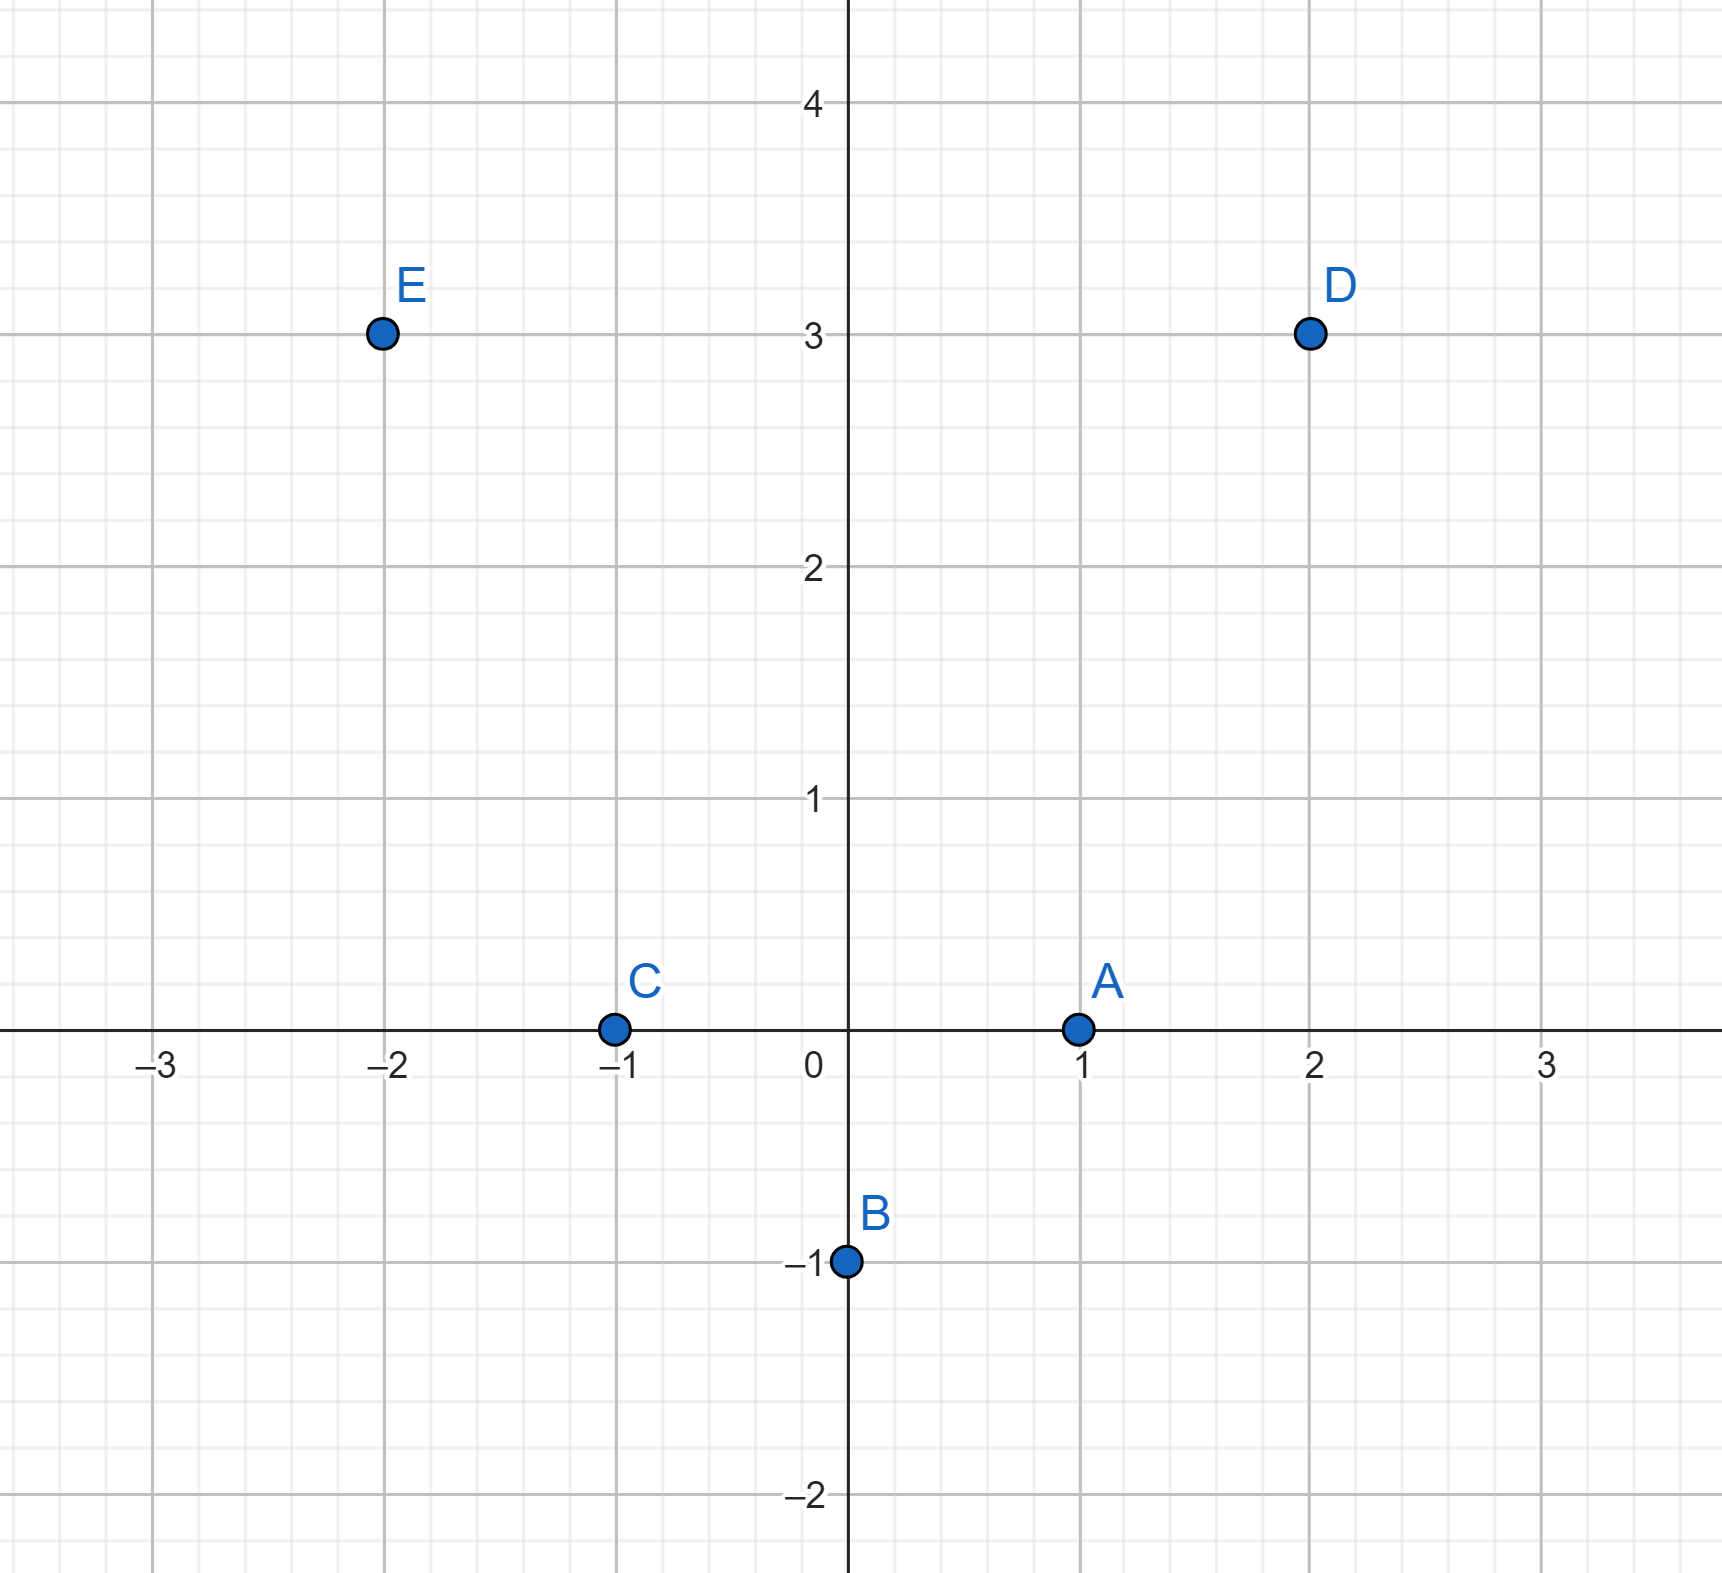
\includegraphics[width=0.34\textwidth]{../figs/Puntos_grafica.png} % Cambia esta ruta por la ubicación de tu imagen
    \caption{Puntos de tabla 1.}
    \label{fig:ejemplo} % Etiqueta para hacer referencia a la imagen
\end{figure}


De esta manera, se puede empezar a representar la grafica de $f$
\begin{figure}[h!] % El entorno figure te permite incluir imágenes
    \centering
    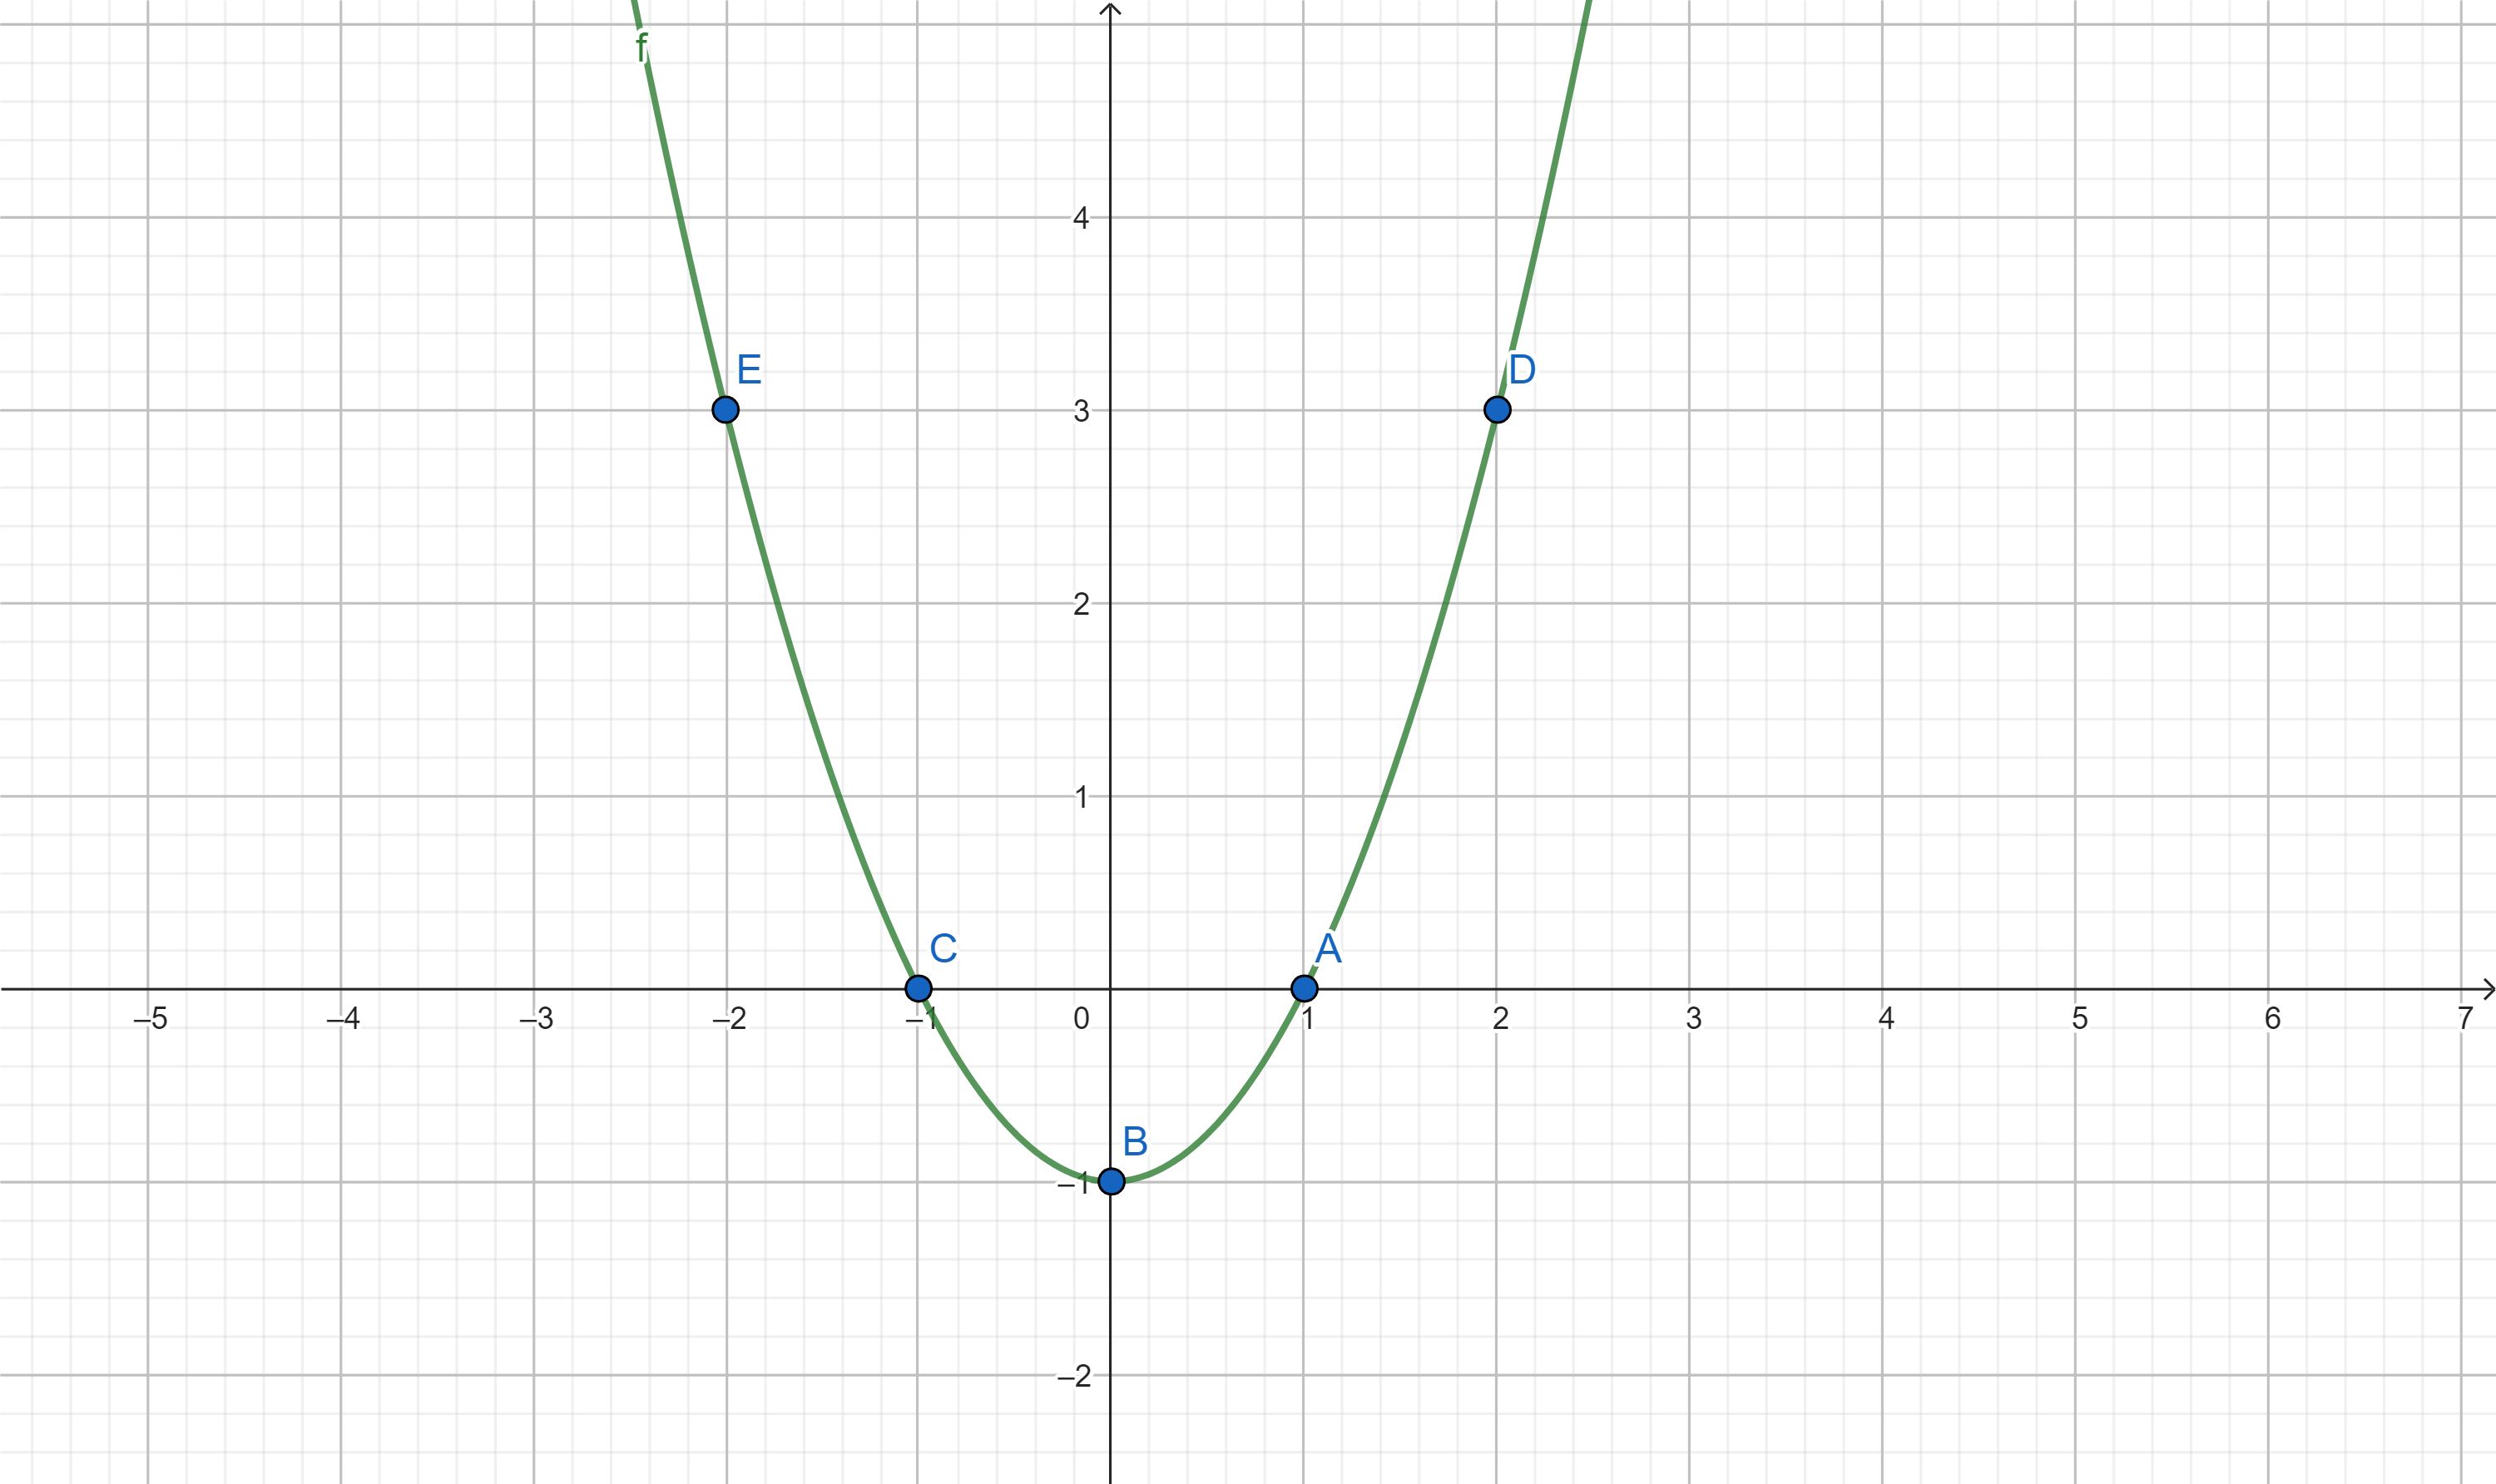
\includegraphics[width=0.5\textwidth]{../figs/r2_grafica.png} % Cambia esta ruta por la ubicación de tu imagen
    \caption{Grafica de $f(x)$.}
    \label{fig:ejemplo} % Etiqueta para hacer referencia a la imagen
\end{figure}
\end{definition}
Ahora, podemos pensar en las mismas definiciones pero analizandolas en $\Re^{3}$, donde la $graf (h)$ de una funcion $h: A\subseteq\Re^{2}\rightarrow\Re$ se define como
 \[
graf(h)=\{(x,y,z)\in\Re^2 \backslash (x,y)\subseteq A=Dom(h) \land z=h(x,y) \}
 \]
En este curso, se analizaran las graficas de funciones en  $\Re^{3}$. Analizamos un ejemplo, tomando $h(x,y)=x^2+y^2$.
Para la función , que representa un paraboloide, los conjuntos de nivel están dados por $h(x,y)=c$, que son círculos concéntricos en el plano xy. Graficando esta función en 3D, podemos ver una superficie parabólica, donde los conjuntos de nivel son las proyecciones de estas circunferencias a diferentes alturas en el eje z y con radio creciente.
\begin{figure}[h!] % El entorno figure te permite incluir imágenes
    \centering
    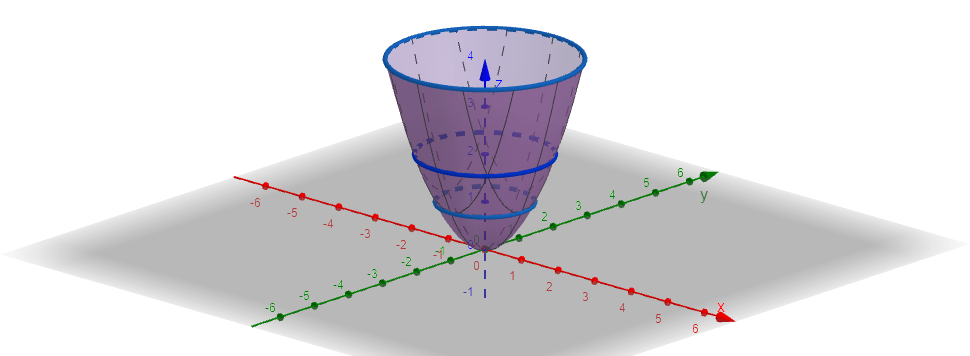
\includegraphics[width=1\textwidth]{../figs/r3_grafica.png} % Cambia esta ruta por la ubicación de tu imagen
    \caption{\small{ Gráfica de h y conjuntos de nivel tomando 
    c=\{1,2,4}\}}
    \label{fig:ejemplo} % Etiqueta para hacer referencia a la imagen
\end{figure}

